% ============================================================
% PASTE THIS OVER THE ENTIRE CONTENT OF main.tex IN OVERLEAF
% Keep preamble.tex and main.bib from the template as-is.
% Upload v13_qualitative.png to the project root.
% Add the entries from main_bib_additions.bib to main.bib.
% ============================================================

\documentclass[sigconf]{acmart}
\input{preamble}

% TikZ for pipeline diagram
\usepackage{tikz}
\usetikzlibrary{arrows.meta,fit,positioning}

\guideStylefalse   % <-- disables grey guide text

\begin{document}

% ---- Author block ----
\author{Mauro Frank Lima de Lima}
\affiliation{%
  \institution{Independent Researcher}
  \city{Market Harborough}
  \country{United Kingdom}
}
\email{mauro.frank.lima@outlook.com}

% ---- Title (keep subtitle from template) ----
\title{Solar Filament Segmentation with U-Net and ResNet34}
\subtitle{A Solution to the Solar Filament Segmentation Challenge 2026}

% ---- Abstract: first sentence is FIXED (black text in template) ----
\begin{abstract}
This report describes our solution to the Solar Filament Segmentation Challenge~2026, a Kaggle competition on automatic segmentation of solar filaments in GONG H-$\alpha$ observations.
We train a U-Net with a ResNet34 encoder on MAGFiLO images resized to 1024$\times$1024 pixels, using random 512$\times$512 crops, Dice loss, and weighted binary cross-entropy (positive class weight~20). Inference applies a single forward pass per image followed by component-wise probability filtering. The v13 checkpoint achieved a crop-level validation Dice of 0.6275 and a public leaderboard score of 0.28. The submitted CSV contains 1,790 instances from 178 of 180 test images.
\end{abstract}

\keywords{solar filaments, H-alpha, U-Net, panoptic quality, MAGFiLO}

\maketitle

% ============================================================
\section{Introduction}
% ============================================================

This report goes over the details of our submitted solution to the Solar Filament Segmentation Challenge~2026 \cite{filament-segmentation-2026}. The challenge, launched on July~10,~2026, is organized by the Earth-Space AI Research (ESAIR) Lab\footnote{\href{https://www.esairlab.com/home}{www.esairlab.com/}}. This challenge utilizes the MAGFiLO dataset for evaluation of the segmentation algorithms \cite{ahmadzadeh2024dataset}.

Our approach converts a foreground probability map into individual instances using thresholding, morphological closing, and connected components. The primary competition metric is Panoptic Quality (PQ)~\cite{kirillov2019panoptic}. No v13 validation PQ was measured; the crop-level Dice reported here is a separate diagnostic. The v13 experiment changed input resolution, training crops, loss weighting, and inference resolution relative to v12; since these changes were not tested in controlled ablations, their individual contributions are unknown.

% ============================================================
\section{Methodology}
% ============================================================

\subsection{Pipeline Overview}

Figure~\ref{fig:pipeline} shows the end-to-end data flow from raw
2048-pixel H-alpha images to the submitted RLE instances.

\begin{figure}[h]
\centering
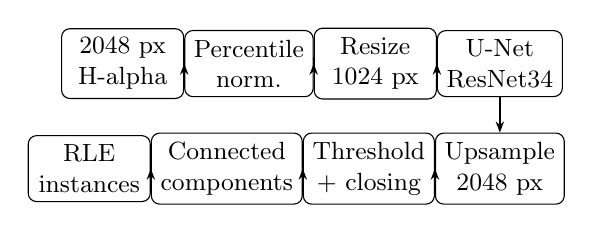
\begin{tikzpicture}[
  box/.style={draw, rounded corners=3pt, minimum width=1.55cm,
              minimum height=0.55cm, align=center, font=\small},
  arr/.style={-{Stealth[length=4pt]}, thick},
  node distance=0.22cm and 0.0cm
]
\node[box] (raw)   {2048 px\\H-alpha};
\node[box, right=of raw]  (norm)  {Percentile\\norm.};
\node[box, right=of norm] (res)   {Resize\\1024 px};
\node[box, right=of res]  (unet)  {U-Net\\ResNet34};
\node[box, below=0.45cm of unet]  (up)    {Upsample\\2048 px};
\node[box, left=of up]    (thr)   {Threshold\\+ closing};
\node[box, left=of thr]   (cc)    {Connected\\components};
\node[box, left=of cc]    (rle)   {RLE\\instances};
\draw[arr] (raw)  -- (norm);
\draw[arr] (norm) -- (res);
\draw[arr] (res)  -- (unet);
\draw[arr] (unet) -- (up);
\draw[arr] (up)   -- (thr);
\draw[arr] (thr)  -- (cc);
\draw[arr] (cc)   -- (rle);
\end{tikzpicture}
\caption{End-to-end inference pipeline. Training uses the same
preprocessing (left half) with random 512-pixel crops and
augmentation.}
\label{fig:pipeline}
\end{figure}

\subsection{Data and Preprocessing}

Images are 2048$\times$2048 grayscale H-alpha JPEGs. Preprocessing:
(1)~convert to grayscale; (2)~normalize intensities to the 1st--99th
percentile range; (3)~resize to 1024$\times$1024. Training masks are
rasterized from COCO polygon annotations. The dataset is split 80/20
by image file (seed~0), giving 918 training and 236 validation items.
Category~4 (Ambiguous) is excluded; the remaining three categories
are merged into one foreground class.

\subsection{Model and Training}

The architecture is \texttt{smp.Unet("resnet34",
in\_channels=1)}~\cite{ronneberger2015unet,he2016resnet}. Training
configuration: Dice loss (smooth\,=\,1) + BCE with
\texttt{pos\_weight=20}; AdamW, $\mathrm{lr}=5\times10^{-4}$;
batch~4; 35 epochs (best at epoch~33); 3-epoch linear warm-up then
cosine decay; fp16 + GradScaler; gradient clip 1.0. Augmentation:
random horizontal/vertical flip and 90-degree rotation.

Validation Dice is computed at threshold 0.5 on random 512-pixel
crops from the resized validation images. It is a crop-level
diagnostic, not a full-image or instance-level metric.

\subsection{Inference and Post-processing}

Each test image is resized to 1024$\times$1024 and processed by one
forward pass (no TTA). The probability map is upsampled to
2048$\times$2048 with bilinear interpolation. A seed mask is formed
at $t_{\mathrm{lo}}=0.35$ and closed with a 5$\times$5 elliptical
kernel. A connected component is retained as one instance when:
peak probability $>0.50$, mean probability $\geq0.30$, and area
$\geq50$ pixels~\cite{afshar2026}. All thresholds are fixed; no
per-image adjustment is applied.

% ============================================================
\section{Evaluation}
% ============================================================

\subsection{Results}

\begin{table}[h]
\caption{v13 submission summary.}
\label{tab:results}
\begin{tabular}{lc}
\toprule
Quantity & Value \\
\midrule
Test images processed    & 180 \\
Images with predictions  & 178 \\
Predicted instances      & 1\,790 \\
TTA                      & No \\
Training resolution      & $1024\times1024$ (crop $512^2$) \\
Output resolution        & $2048\times2048$ \\
Val.\ crop Dice (ep.\ 33) & 0.6275 \\
Public leaderboard score & 0.28 \\
\bottomrule
\end{tabular}
\end{table}

The v12 submission scored 0.00 due to overly restrictive default
thresholds ($t_{\mathrm{hi}}=0.99$, $\mathrm{min\_meanp}=0.85$)
that suppressed all predictions. The v13 result of 0.28 reflects
corrected thresholds and a retrained model; the individual
contribution of each change is unknown.

\subsection{Qualitative Predictions}

Figure~\ref{fig:qualitative} shows three test images with different
instance counts. Colors distinguish RLE instances; no ground-truth
comparison is available for test images.

\begin{figure}[h]
\centering
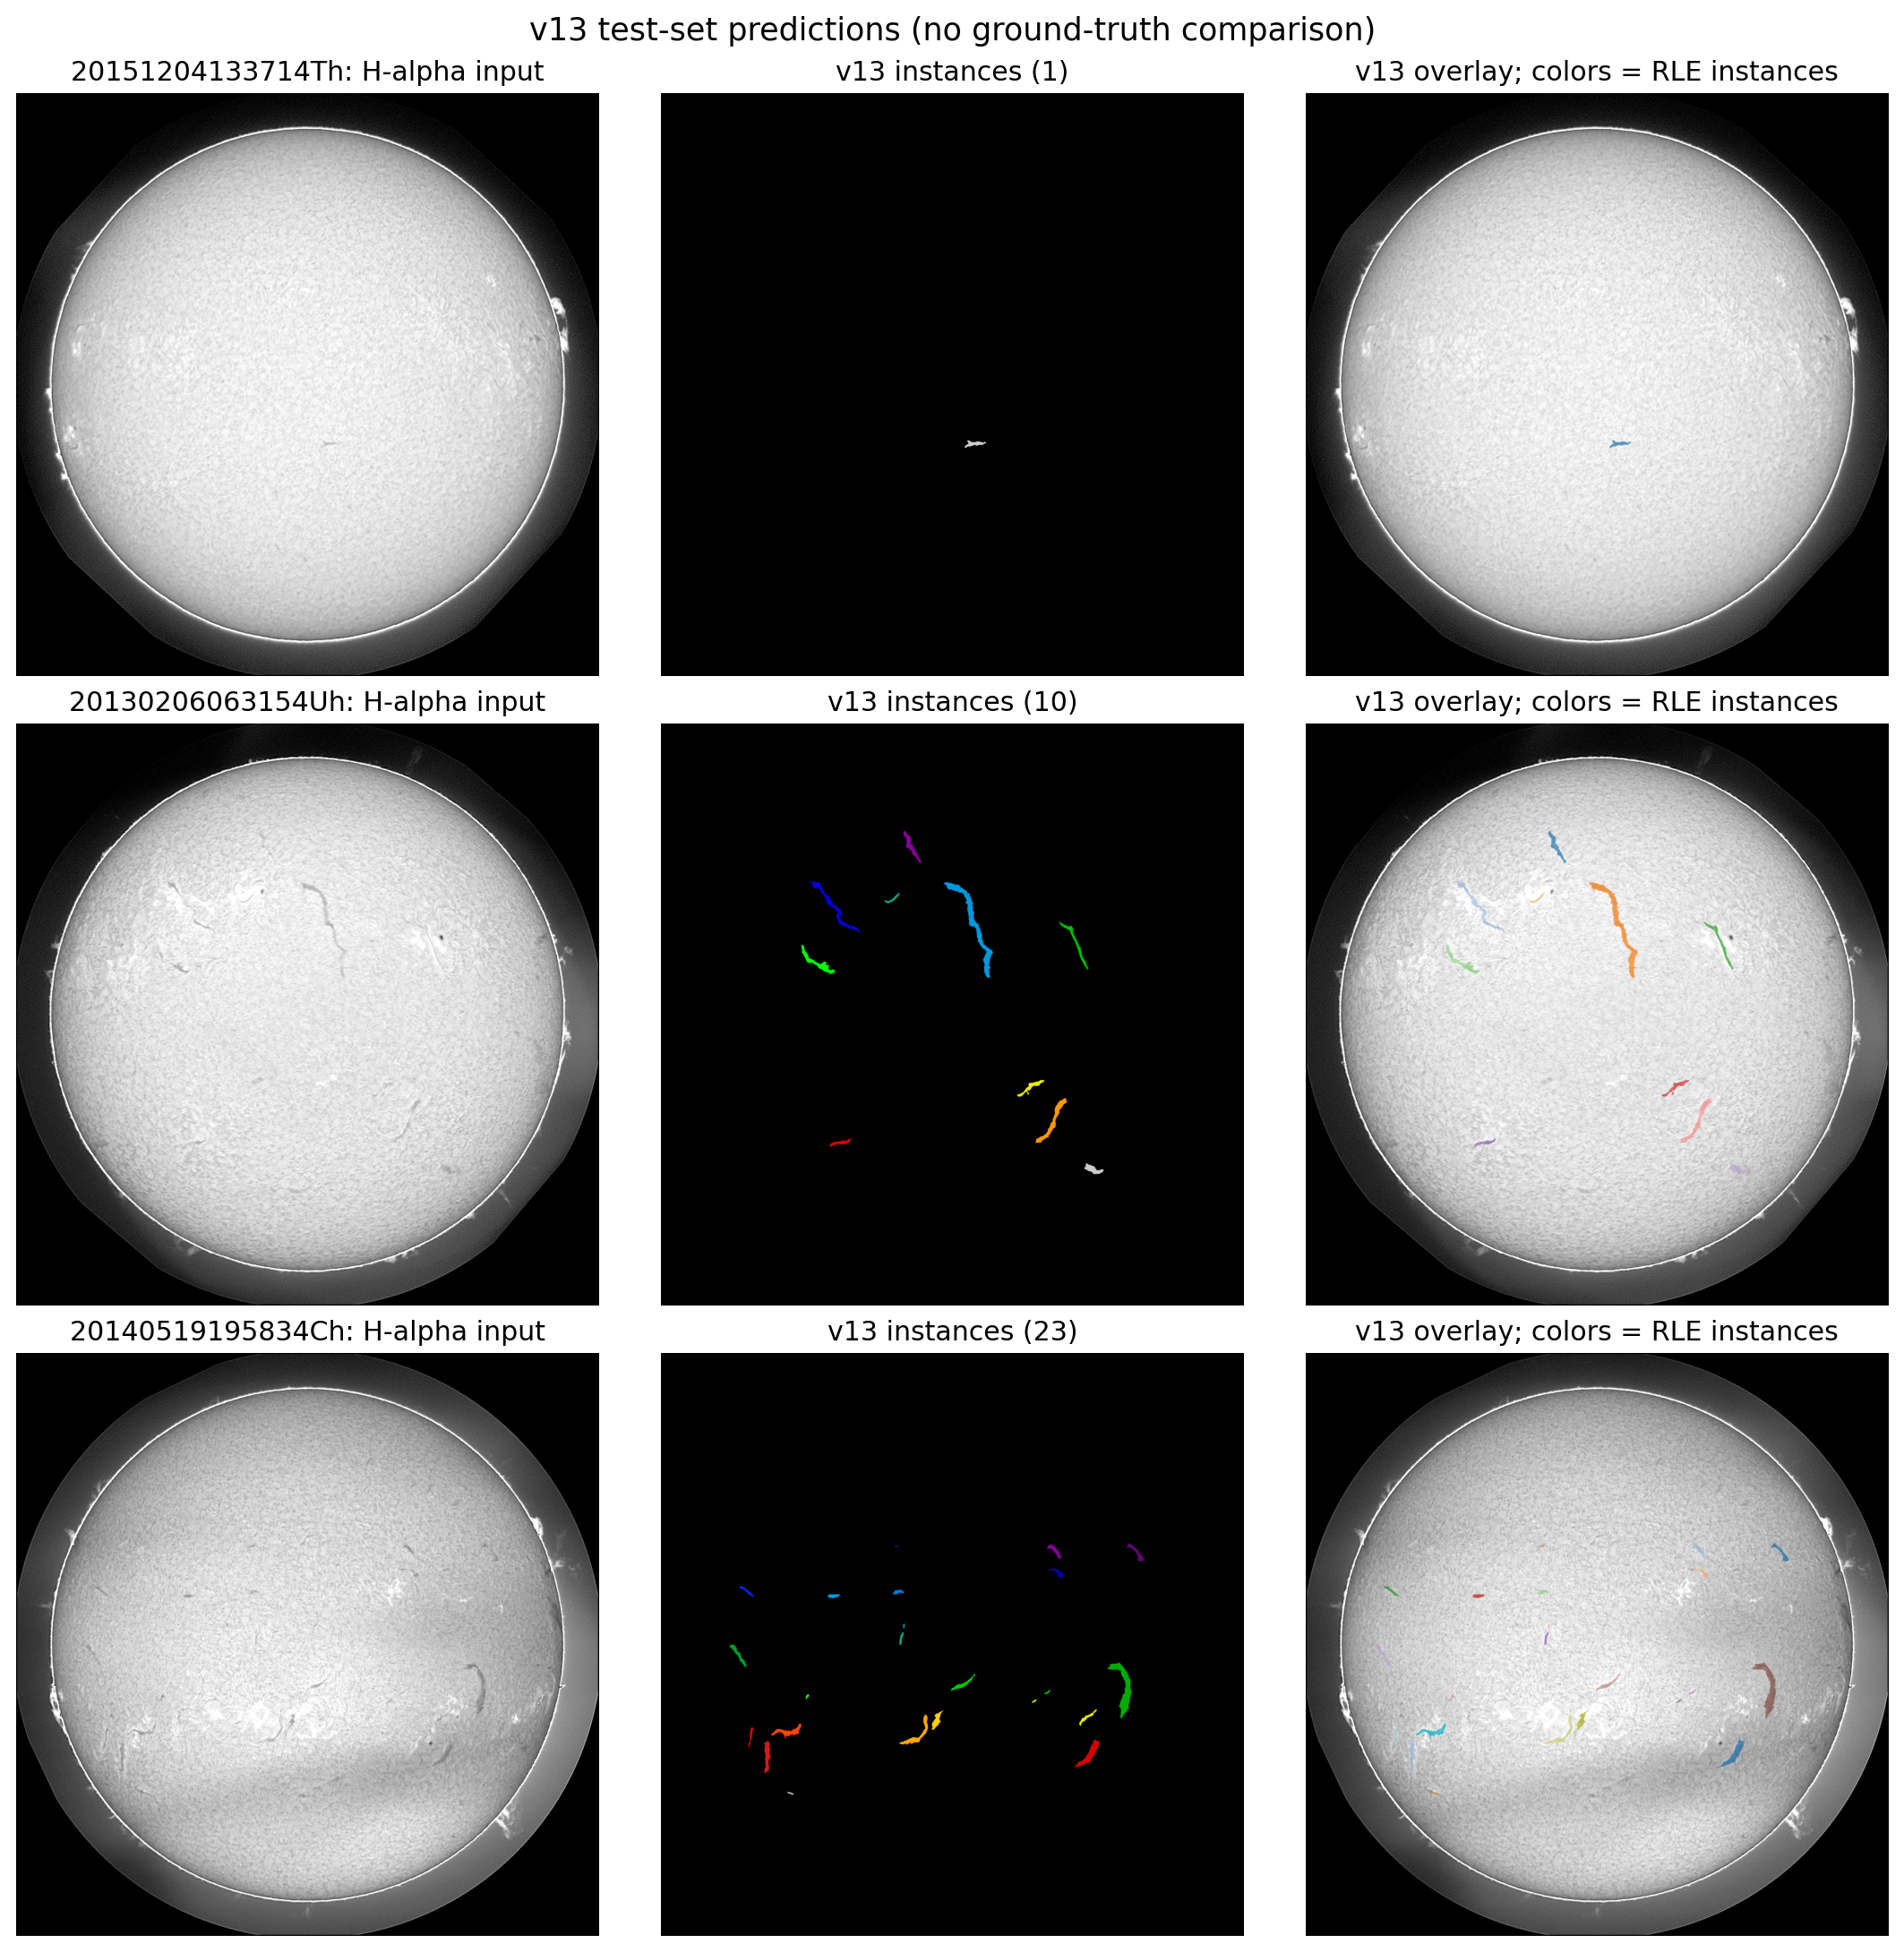
\includegraphics[width=\columnwidth]{v13_qualitative.png}
\caption{v13 predictions on test images 20151204133714Th (1 retained
instance), 20130206063154Uh (10), and 20140519195834Ch (23). Each
row shows the H-alpha input, predicted instances, and overlay.
Colors distinguish instances. Test ground truth was not available.}
\label{fig:qualitative}
\end{figure}

\subsection{Strengths, Weaknesses, and Improvements}

\textbf{Strengths.} The pipeline is simple and fully reproducible:
fixed thresholds, no TTA, one checkpoint. The ResNet34 encoder
provides strong pretrained features for a single-channel input.

\textbf{Weaknesses.} No v13 validation PQ was measured. Two test
images have no predictions. Resizing to 1024 px reduces spatial
detail; random crops expose the model to local regions rather than
the full solar disk. The fixed thresholds were not selected by a
completed PQ sweep on v13 weights. Merging three annotation
categories into one foreground class discards category distinctions.

\textbf{Improvements.} Full-image instance PQ on a held-out
validation set would enable principled threshold selection. TTA,
larger input resolution, and multi-scale training are natural next
steps. A controlled ablation varying one setting at a time would
clarify which changes drive the score.

\subsection{Reproducibility}

Code, weights (\path{weights/best.pt}, float32, 97.9\,MB), and
inference notebook (\path{pipeline.ipynb}) are at:
\begin{center}
\url{https://github.com/maurolima-sys/solar-filament-segmentation}
\end{center}
Install with \texttt{pip install -r requirements.txt} and run
\path{pipeline.ipynb}. The notebook loads \path{weights/best.pt}
without retraining and writes \path{submission\_v13.csv}. The exact
CSV is included in the repository. Training used a Kaggle T4 GPU;
inference runs on CPU or GPU.

% ============================================================
% ACKNOWLEDGMENT — DO NOT CHANGE (official template text)
% ============================================================
\section{Acknowledgment}\label{sec:acknowledgment}
The organization of the Filament Segmentation Challenge 2026 is partially supported by the U.S. National Science Foundation (NSF) under Grant No. 2209912 and 2433781, directorate for Computer and Information Science and Engineering (CSE), and Office of Advanced Cyberinfrastructure (OAC), and Grant No. 2511630, AST Division Of Astronomical Sciences and MPS Directorate for Mathematical and Physical Sciences.

The Filament Segmentation Challenge 2026 is sponsored by the U.S. National Science Foundation (NSF) National Solar Observatory (NSO).

This work utilizes GONG data obtained by the NSO Integrated Synoptic Program, managed by the National Solar Observatory, which is operated by the Association of Universities for Research in Astronomy (AURA), Inc. under a cooperative agreement with the National Science Foundation and with contribution from the National Oceanic and Atmospheric Administration. The GONG network of instruments is hosted by the Big Bear Solar Observatory, High Altitude Observatory, Learmonth Solar Observatory, Udaipur Solar Observatory, Instituto de Astrofísica de Canarias, and Cerro Tololo Interamerican Observatory.

\bibliographystyle{ACM-Reference-Format}
\bibliography{main}

\end{document}
